\chapter{\ac{HMM}}
\section{Construction}
La construction de la structure de base pour le HMM implique de créer un modèle
par classe du problème. Dans notre cas, nous voulons déterminer l'état d'une batterie,
à savoir bonne, moyenne ou mauvaise. Pour cela, nous avons à disposition des mesures
de charges et décharges.

Nous avons donc besoin de 6 modèles au total, 3 pour la charge et 3 pour la décharge.

Comme la qualité des batteries ne peux que se dégrader ou rester stable, le \ac{HMM} est de type gauche-droite.

\subsection{Modèle}
Les modèles sont construit avec les mêmes paramètres de départ qui sont:
\begin{itemize}
    \item un vecteur de probabilité de départ.
    \item une matrice de transport.
    \item le nombre de composants.
    \item le nombre d'itération.
\end{itemize}

\begin{minted}{python}
model = hmm.GaussianHMM(verbose=verb, n_iter=it, n_components=N, init_params='st')
model.startprob_ = np.zeros(N)
model.startprob_[0] = 1
model.transmat_ = (np.identity(N) + np.diagflat(np.ones(N - 1), 1)) * 0.5
model.transmat_[-1, -1] = 1
\end{minted}
Le vecteur startprob est de la forme [1,0,....,0]. Car une batterie démarre toujours
dans un état initial connu.

La matrice transmat permet un transfert de l'état actuel à lui-même ainsi qu'à
l'état suivant avec une probabilité de 50\% sauf pour le dernier état qui reste
obligatoirement lui-même.

\subsection{Prédiction}
Afin de choisir l'état de la batterie, nous utilisons le score de chaque modèle.
Nous faisons une prédiction pour le cycle de charge ainsi que pour la décharge.
Le score maximum nous donne l'état de la batterie testée.

\begin{minted}{python}
def get_predict(features, models):
    predict = []
    nb_feat = features.shape[1]
    length = features.shape[0]
    for i in range(length):
        score = []
        for model in models:
            score.append((model.score(np.array(features.iloc[i, :]).reshape(1, nb_feat))))
        predict.append(np.argmax(score) + 1)
    return predict
\end{minted}

Puis nous fusionnons les scores en utilisant le maximum des deux prédictions.
Ce choix a été motivé par les scores des modèles que nous verrons plus bas.

\begin{minted}{python}
lenMax = max(len(predict_cha), len(predict_dis))
lenMin = min(len(predict_cha), len(predict_dis))
res = []
for i in range(lenMax):
    if i >= lenMin:
        res.append(predict_cha[i])
    else:
        res.append(max((predict_dis[i], predict_cha[i])))
\end{minted}

\subsection{Scores}
Pour évaluer la qualité de la prédiction, nous avons utilisé le nombre de prédiction
juste, le F1 score ainsi que la matrice de confusion. Le nombre de prédiction
permettait d'observer un résultat dans les cas où le modèle choisissait un seul et
unique résultat.

\section{Traitement des données}
Des données importées, nous supprimons les références à la date et l'heure de mesure car cela n'est pas présent dans l'ensemble de test.
Nous séparons ensuite les cycles de charge et de décharge pour les traiter.

Les mesures ont des sauts importants au début comme le montre la figure \ref{fig:courFull}. Afin que cela n'influence pas la prédiction les 2 premiers éléments de chaque mesure sont supprimés. La figure \ref{fig:courTron} montre le résultat qui est utilisé pour calculer les features.
\begin{figure}
    \centering
    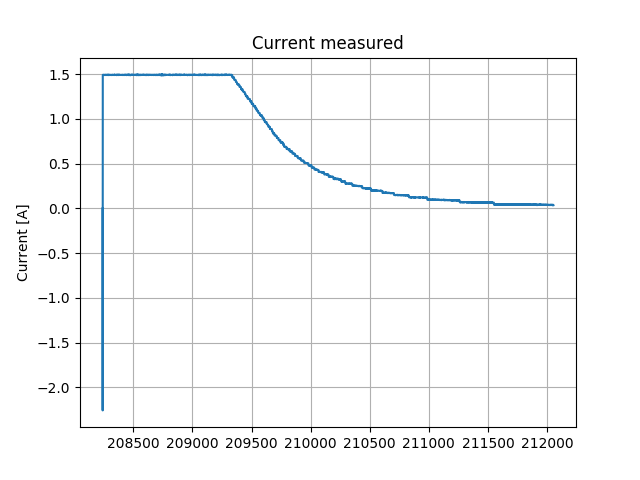
\includegraphics[scale=0.5]{images/currentmeas.png}
    \caption{Courant mesuré complet}
    \label{fig:courFull}
\end{figure}

\begin{figure}
    \centering
    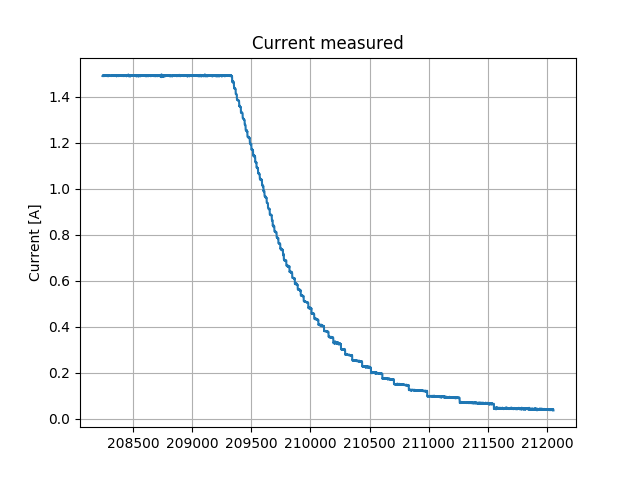
\includegraphics[scale=0.5]{images/currentmeasfilt.png}
    \caption{Courant mesuré tronqué}
    \label{fig:courTron}
\end{figure}

Pour extraire les features, nous séparons chaque cycle de chaque batterie. 

\section{Choix des features}
Les features ont été sélectionnées grâce à une répétition de test pour observer laquelle
apportait le plus au modèle.

\subsection{Charge}
Les features sélectionnées pour la charge sont les suivantes:
- Le maximum de la tension mesurée
- Le 25\ieme centile de la tension mesurée
- Le 25\ieme centile du courant mesuré
- La médiane de la température mesurée
- Le 25\ieme centile de la température mesurée
- Le maximum de la différence entre deux mesures de la température

\subsection{Décharge}
Les features sélectionnées pour la décharge sont les suivantes:
- Le minimum de la capacité
- Le maximum de la tension mesurée

\section{Choix des paramètres}
Pour sélectionner les meilleurs paramètres, le nombre d'éléments et d'itérations ont été essayé de manière croisée avec des valeurs allant de 3 à 20.
Le choix s'est porté sur la combinaison qui donnait le meilleur score.
Le meilleur résultat a été obtenu pour dix itérations et 5 composants.

\section{Résultats}
\subsection{Charge}
Pour un modèle ne prenant en compte que la charge, nous obtenons la matrice de confusion de la figure \ref{fig:HMMconfCha}

\begin{figure}
    \centering
    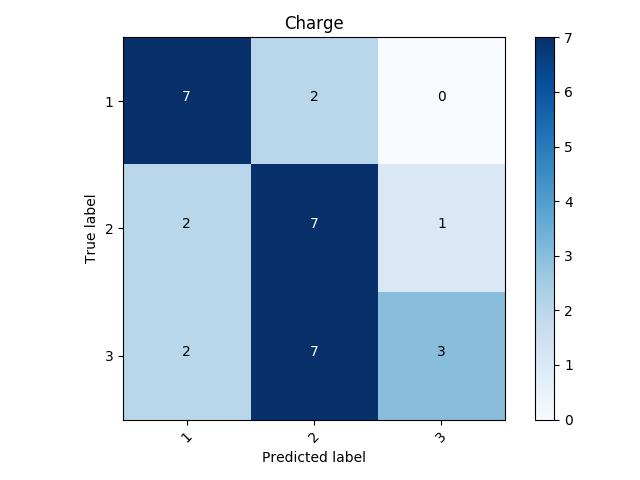
\includegraphics[scale=0.5]{images/Confcha.png}
    \caption{Matrice de confusion pour la charge}
    \label{fig:HMMconfCha}
\end{figure}

\begin{figure}
    \centering
    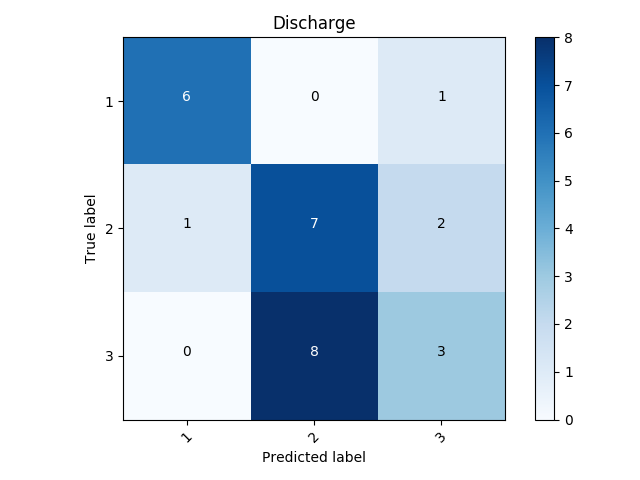
\includegraphics[scale=0.5]{images/Confdech.png}
    \caption{Matrice de confusion pour la décharge}
    \label{fig:HMMconfDecha}
\end{figure}

\begin{figure}
    \centering
    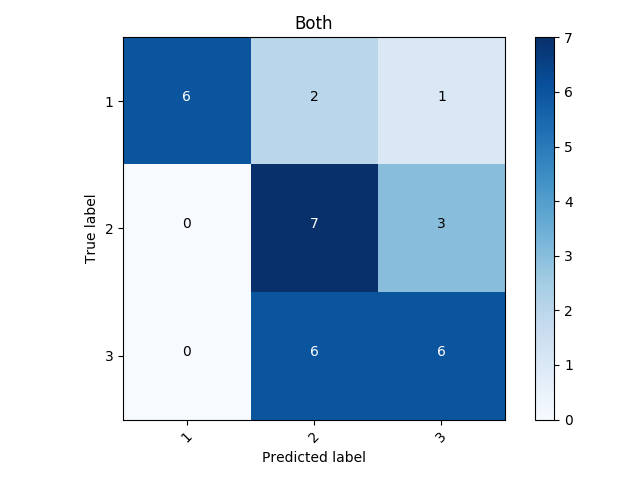
\includegraphics[scale=0.5]{images/Confboth.png}
    \caption{Matrice de confusion pour les deux cycles}
    \label{fig:HMMconfboth}
\end{figure}